\documentclass[a4paper]{article}
\usepackage[francais]{babel}
\usepackage{fontspec}
\usepackage{enumitem}
\usepackage{authblk}
\usepackage{minted}
\usepackage{amsmath}
\usepackage{tabularx}
\newcolumntype{C}[1]{>{\centering\arraybackslash}p{#1}}
\graphicspath{{images/}}
\setlength{\parindent}{0pt}
\usepackage[left=2.5cm,top=2.5cm,right=2.5cm,bottom=2.5cm]{geometry}
 
\title{Projet VHDL}
\author{Mehmed Blazevic \& Orphée Antoniadis}
\date{Hepia 2018}
\begin{document}

\maketitle

\section{Introduction}
Dans le cadre du cours de VHDL, FPGA \& SoPC, il nous a été demandé de réaliser un projet. 
Le projet s'étale sur tout le semestre et le thème est libre. Nous avions tout de 
même certaines contraites:

\begin{itemize}
  \item Utiliser un périphérique existant (SPI, I2C, UART, ...)
  \item Créer un périphérique spécifique
\end{itemize}

\section{Notre idée}
Nous voulions travailler avec le musique. On pensait faire un instrument un peu 
différent de ce que l'on a l'habitude de voir. L'idée est de travailler avec l'espace. 
Nous avons décidé d'utiliser des capteurs ultrasons, afin de connaître la distance 
entre une main et ce capteur. En fonction de la distance que l'on mesure avec la main, 
nous avions dans l'idée de produire une notes de musique plus ou moins forte. 
L'idée était de placer 8 capteurs de distances allignés, afin de jouer avec un piano 
"virtuel". 

\subsection{Schema}

\begin{center}
\noindent\makebox[\textwidth]{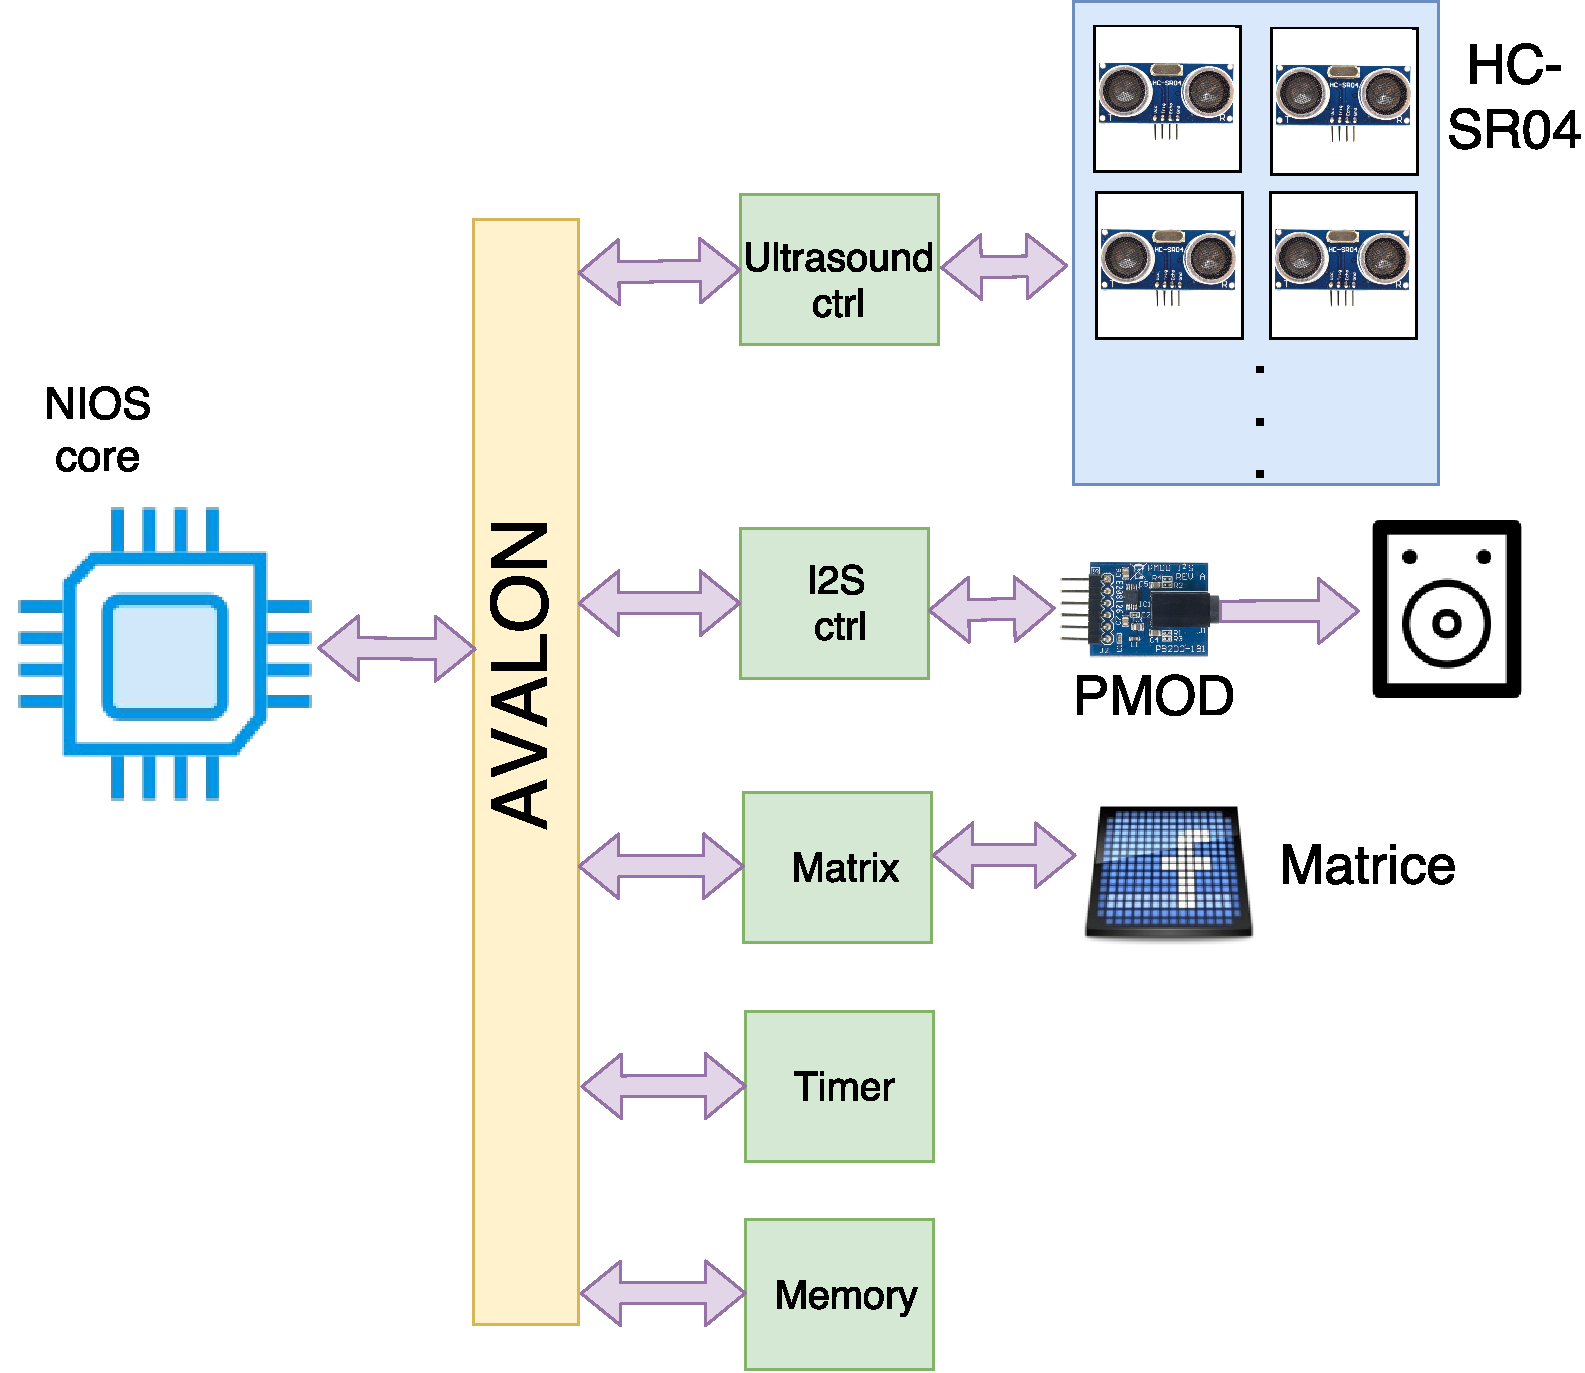
\includegraphics[width=350pt]{VHDL.pdf}}
\end{center}

\end{document}
